\documentclass{beamer}

\usepackage{beamerthemesplit}
\usepackage[utf8x]{inputenc}
\usepackage{pgf}
\usepackage{default}
\usepackage{url}
\usepackage{subfigure}
\usepackage{algorithmic} 
\usepackage{algorithm} 
\usepackage{amssymb}
\usepackage{graphicx}
\usepackage{booktabs}
\usepackage{mathtools}

\usetheme{Singapore}


%Define some commands for printing correct variables in math mode 
\newcommand{\av}{\textbf{a}}
\newcommand{\bv}{\textbf{b}}
\newcommand{\cv}{\textbf{c}}
\newcommand{\dv}{\textbf{d}}
\newcommand{\ev}{\textbf{e}}
\newcommand{\fv}{\textbf{f}}
\newcommand{\gv}{\textbf{g}}
\newcommand{\hv}{\textbf{h}}
\newcommand{\iv}{\textbf{i}}
\newcommand{\jv}{\textbf{j}}
\newcommand{\kv}{\textbf{k}}
\newcommand{\lv}{\textbf{l}}
\newcommand{\mv}{\textbf{m}}
\newcommand{\nv}{\textbf{n}}
\newcommand{\ov}{\textbf{o}}
\newcommand{\pv}{\textbf{p}}
\newcommand{\qv}{\textbf{q}}
\newcommand{\rv}{\textbf{r}}
\newcommand{\sv}{\textbf{s}}
\newcommand{\tv}{\textbf{t}}
\newcommand{\uv}{\textbf{u}}
\newcommand{\vv}{\textbf{v}}
\newcommand{\wv}{\textbf{w}}
\newcommand{\xv}{\textbf{x}}
\newcommand{\yv}{\textbf{y}}
\newcommand{\zv}{\textbf{z}}

\newcommand{\alphav}{\mbox{\boldmath$\alpha$}}
\newcommand{\betav}{\mbox{\boldmath$\beta$}}
\newcommand{\gammav}{\mbox{\boldmath$\gamma$}}
\newcommand{\xiv }{\mbox{\boldmath$\xi$}}
\newcommand{\muv}{\mbox{\boldmath$\mu$}}
\newcommand{\tauv}{\mbox{\boldmath$\tau$}}
\newcommand{\Omegam}{\mbox{\boldmath$\Omega$}}
\newcommand{\Lambdam}{\mbox{\boldmath$\Lambda$}}
\newcommand{\Sigmam}{\mbox{\boldmath$\Sigma$}}
\newcommand{\Gammam}{\mbox{\boldmath$\Gamma$}}
\newcommand{\Deltam}{\mbox{\boldmath$\Delta$}}
\newcommand{\Thetam}{\mbox{\boldmath$\Theta$}}
\newcommand{\Phim}{\mbox{\boldmath$\Phi$}}
\newcommand{\Pim}{\mbox{\boldmath$\Pi$}}

\newcommand{\diag}{\mbox{diag}}
\newcommand{\tr}{\mbox{tr}}
\newcommand{\card}{\mbox{card}}
\newcommand{\cov}{\mbox{cov}}
\newcommand{\sign}{\mbox{sign}}
\newcommand{\var}{\mbox{var}}
\newcommand{\st}{\mbox{s.t.}}
\newcommand{\rank}{\mbox{rank}}
\newcommand{\argmin}{\mbox{argmin}}
\newcommand{\argmax}{\mbox{argmax}}

\newcommand{\Am}{\textbf{A}}
\newcommand{\Bm}{\textbf{B}}
\newcommand{\Cm}{\textbf{C}}
\newcommand{\Dm}{\textbf{D}}
\newcommand{\Em}{\textbf{E}}
\newcommand{\Fm}{\textbf{F}}
\newcommand{\Gm}{\textbf{G}}
\newcommand{\Hm}{\textbf{H}}
\newcommand{\Imat}{\textbf{I}}
\newcommand{\Jm}{\textbf{J}}
\newcommand{\Km}{\textbf{K}}
\newcommand{\Lm}{\textbf{L}}
\newcommand{\Mm}{\textbf{M}}
\newcommand{\Nm}{\textbf{N}}
\newcommand{\Om}{\textbf{O}}
\newcommand{\Pm}{\textbf{P}}
\newcommand{\Qm}{\textbf{Q}}
\newcommand{\Rm}{\textbf{R}}
\newcommand{\Sm}{\textbf{S}}
\newcommand{\Tm}{\textbf{T}}
\newcommand{\Um}{\textbf{U}}
\newcommand{\Vm}{\textbf{V}}
\newcommand{\Wm}{\textbf{W}}
\newcommand{\Xm}{\textbf{X}}
\newcommand{\Ym}{\textbf{Y}}
\newcommand{\Zm}{\textbf{Z}}

%Use regular expression: (\[a-z])([^a-zA-Z])  -> \1v\2  to change old style macros 
\graphicspath{{./Figures/}}

\title{Statistics and the Analysis of Data\\ Lecture 6: Limit Theorems}
\author{Charanpal Dhanjal \\ \texttt{charanpal@gmail.com}} 
\institute{\'{E}cole des Ponts}
\date{7th January 2014}

\begin{document}

\frame{\titlepage}


\begin{frame}{Recap}  
\begin{itemize} 
\item Continuous distributions - uniform, exponential, Gaussian 
\item Random vectors, covariance matrices 
\item The multivariate Gaussian 
\end{itemize}
\end{frame}

\begin{frame}{Outline}  
\begin{itemize} 
 \item We want to know about convergence of random variables 
\begin{itemize}
\item Difference types of convergence 
\item Strong law of large numbers 
\item Central Limit Theorem 
\end{itemize}
\end{itemize}
\end{frame}

\begin{frame}{Almost Sure Convergence}  
\begin{itemize}
 \item Sequence of random variables $X_1, X_2, \ldots$ will \emph{converge almost surely} (i.e. with probability 1) towards $Y$ if there is an event $\Omega_0 \subset \Omega$ with $P(\Omega_0) = 1$ and 
\begin{displaymath}
X_n(\omega) \xrightarrow[n \rightarrow \infty]{} Y(\omega) 
\end{displaymath}
 for all $\omega \in \Omega_0$
\end{itemize}
\end{frame}

\begin{frame}{An Example} 
\begin{itemize}
 \item A man rolls 5 dice every day and donates $N$ Euros to charity where $N$ is the sum of the values on the dice. If the dice are all ones however, he stops permanently.  
 \item Let $X_1, X_2, \ldots$ be the daily amounts the charity receives from him.
 \item We may be almost sure that one day this amount will be zero, and stay zero forever after that.
 \item However, when we consider any finite number of days, there is a nonzero probability the terminating condition will not occur. 
\end{itemize}
\end{frame}

\begin{frame}{Convergence in Mean} 
\begin{itemize}
 \item Consider a sequence of random variables $X_1, X_2, \ldots$ that \emph{converges in mean} to $Y$, $\mathbb{E}[|X_n - Y|^p] \xrightarrow[n \rightarrow \infty]{} 0$ for some fixed $p \geq 1$
 \item We can write this as $X_n \xrightarrow[n \rightarrow \infty]{\mathbb{L}^p} Y$ 
 \item Some properties 
 \begin{itemize} 
  \item If $X_n \xrightarrow[n \rightarrow \infty]{\mathbb{L}^p} Y$ and $X_n' \xrightarrow[n \rightarrow \infty]{\mathbb{L}^p} Y'$ then $X_n + \lambda X_n' \xrightarrow[n \rightarrow \infty]{\mathbb{L}^p} Y + \lambda Y'$ for all $\lambda \in \mathbb{R}$
  \item  If $X_n \xrightarrow[n \rightarrow \infty]{\mathbb{L}^p} Y$ and $X_n' \xrightarrow[n \rightarrow \infty]{\mathbb{L}^p} Y'$  then the following is not necessarily true $X_nX_n' \xrightarrow[n \rightarrow \infty]{\mathbb{L}^p} Y Y'$
 \end{itemize}
\end{itemize} 
\end{frame}

\begin{frame}{Convergence in Probability}  
\begin{itemize} 
 \item Let $Y$ be a continuous random variable and $X_1, X_2, \ldots$ be a sequence of random variables. Then $X_1, X_2, \ldots$ \emph{converges in probability} to $Y$ if 
\begin{displaymath}
\lim_{n \rightarrow \infty} P(|X_n - Y| > \epsilon) = 0
\end{displaymath}
for all $\epsilon > 0$
 \item Convergence almost surely and in mean imply convergence in probability. 
\end{itemize}
\end{frame}

\begin{frame}{An Example} 
\begin{itemize}
 \item Consider a large jar full of water, and let $X$ be the mass of the water in Kg. Note $X$ is a random variable. 
 \item People are asked successively to estimate the mass of the water just by looking at it and let $X_n$ be the mean of the first $n$ responses 
 \item Then the sequence $X_n$ will converge in probability to the random variable $X$ (why?)  
\end{itemize}
\end{frame}

\begin{frame}{Exercise} 
\begin{itemize} 
\item Let $X_1, X_2, \ldots X_n$  be a sequence of discrete random variables. Let the probability mass function of $X_i$ for all $i$ be given by $P(X_i = n) = \frac{1}{n}$ and $P(X_i = 0) = 1-\frac{1}{n}$. 
\item Show whether the mean-square limit exists for the sequence $X_1, X_2, \ldots X_n$
\end{itemize}
\end{frame}

\begin{frame}{Strong Law of Large Numbers} 
\begin{itemize}
 \item Let $X_1, X_2, \ldots X_n$ be a set of i.i.d (independent and identically distributed) random variables that are integrable $\mathbb{E}[X_i] < \infty$ for all $i$
 \item Then as $n \rightarrow \infty$ the \emph{Strong Law of Large Numbers} says
 \begin{displaymath} 
  \bar{X}_n = \frac{1}{n}\sum_{i=1}^n X_i \xrightarrow{a.s.} \mathbb{E}[X_1]
 \end{displaymath}
\item Furthermore 
\begin{displaymath} 
 \bar{X}_n \xrightarrow{\mathbb{L}^2} \mathbb{E}[X_1]
\end{displaymath}
\end{itemize}
\end{frame}

\begin{frame}{An Example}
The expected value of rolling a fair die is 3.5. Let $X_n$ be the mean value after $n$ rolls. 
\begin{figure}[htp]
\mbox{
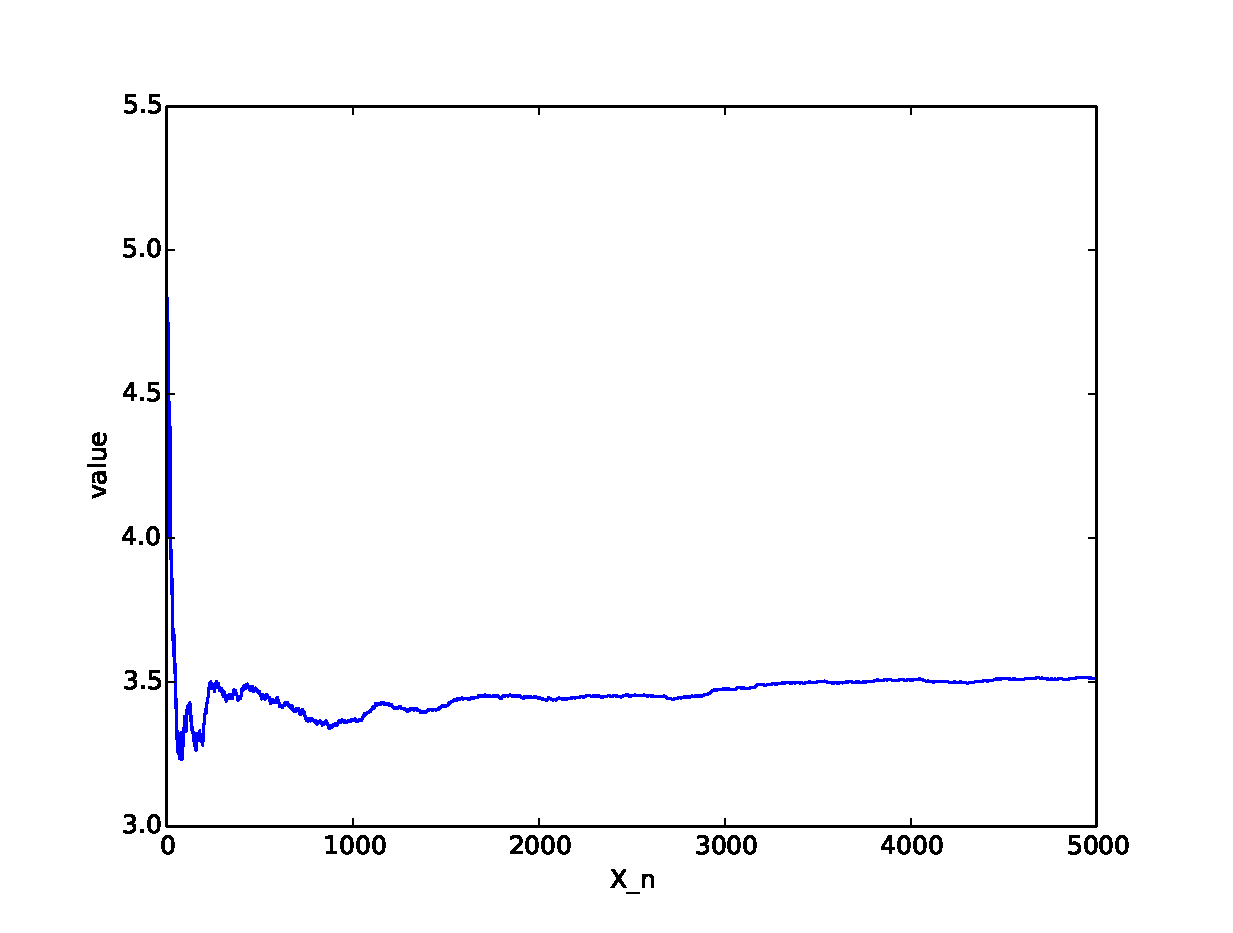
\includegraphics[width=0.5\linewidth]{LawLargeNumbers.eps}
}
\end{figure} 
\end{frame}

\begin{frame}{Central Limit Theorem} 
\begin{itemize} 
 \item Let $X_1, \ldots, X_n$ be a set of $n$ independent and identically distributed variables with mean $\mu$ and nonzero finite variance $\sigma^2$. Let $Y = \sum_{i=1}^n X_i$, then 
\begin{displaymath}
 \mbox{lim}_{n \rightarrow \infty} P\left(\frac{Y - n\mu}{\sigma\sqrt{n}} \leq x\right) = \phi(x)
\end{displaymath}
where $\phi$ is the cumulative distribution function for the standard normal distribution. 
\item In other words, $Y$ tends towards a normal distribution regardless of the distribution of $X_i$'s 
\end{itemize}
\end{frame}

\begin{frame}{An Example}  
\begin{itemize} 
 \item Generate $n$ uniform random variables $X_1, \ldots, X_n \sim \mathcal{U}(1, 2)$ 
\item Sample from $Y = \sum_{i=1}^n \frac{X_i - n\mu}{\sigma \sqrt{n}}$ 
\end{itemize}
 \begin{figure}[htp]
\mbox{
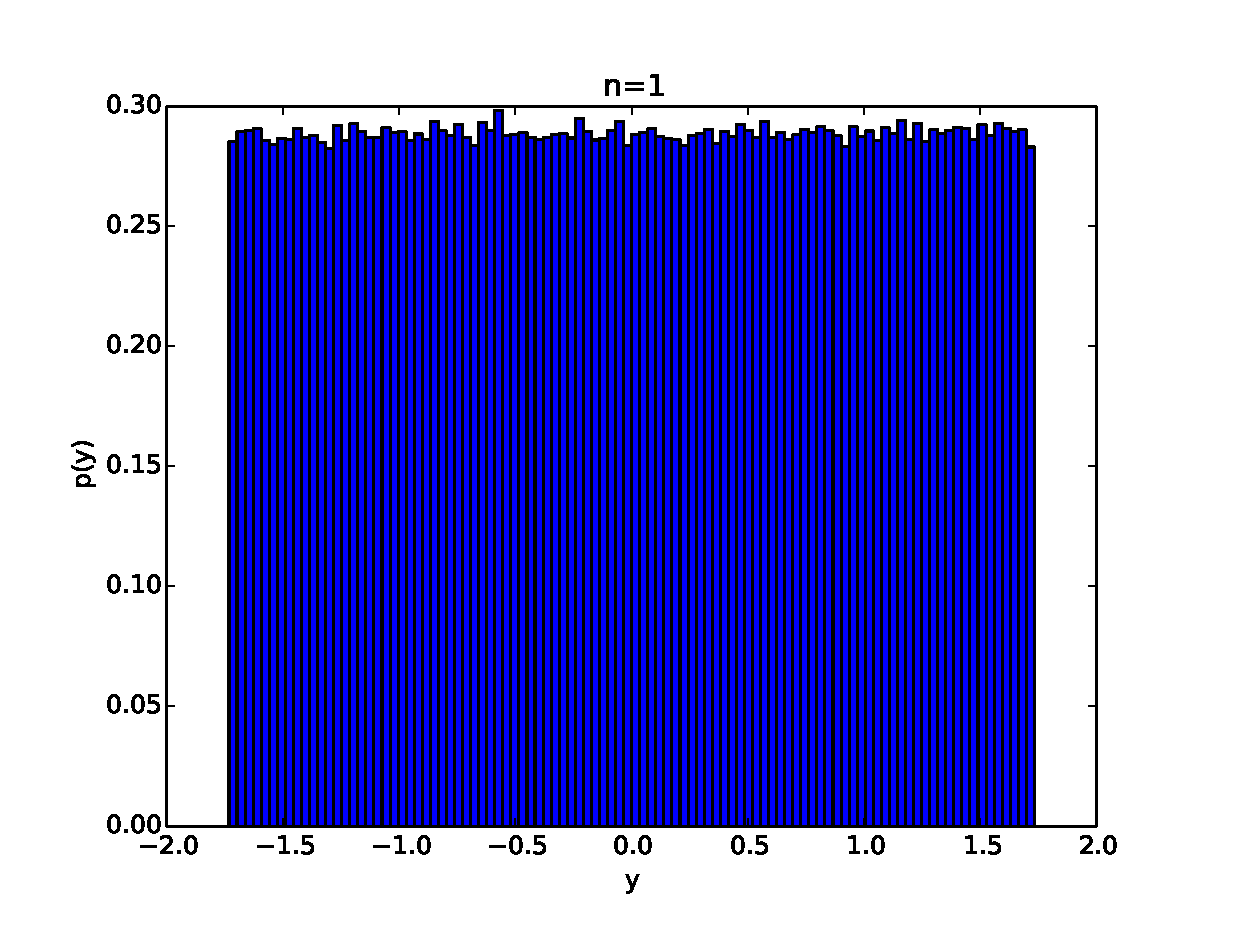
\includegraphics[width=0.5\linewidth]{clt0.eps}
}
\end{figure} 
\end{frame}

\begin{frame} 
  \begin{figure}[htp]
\mbox{
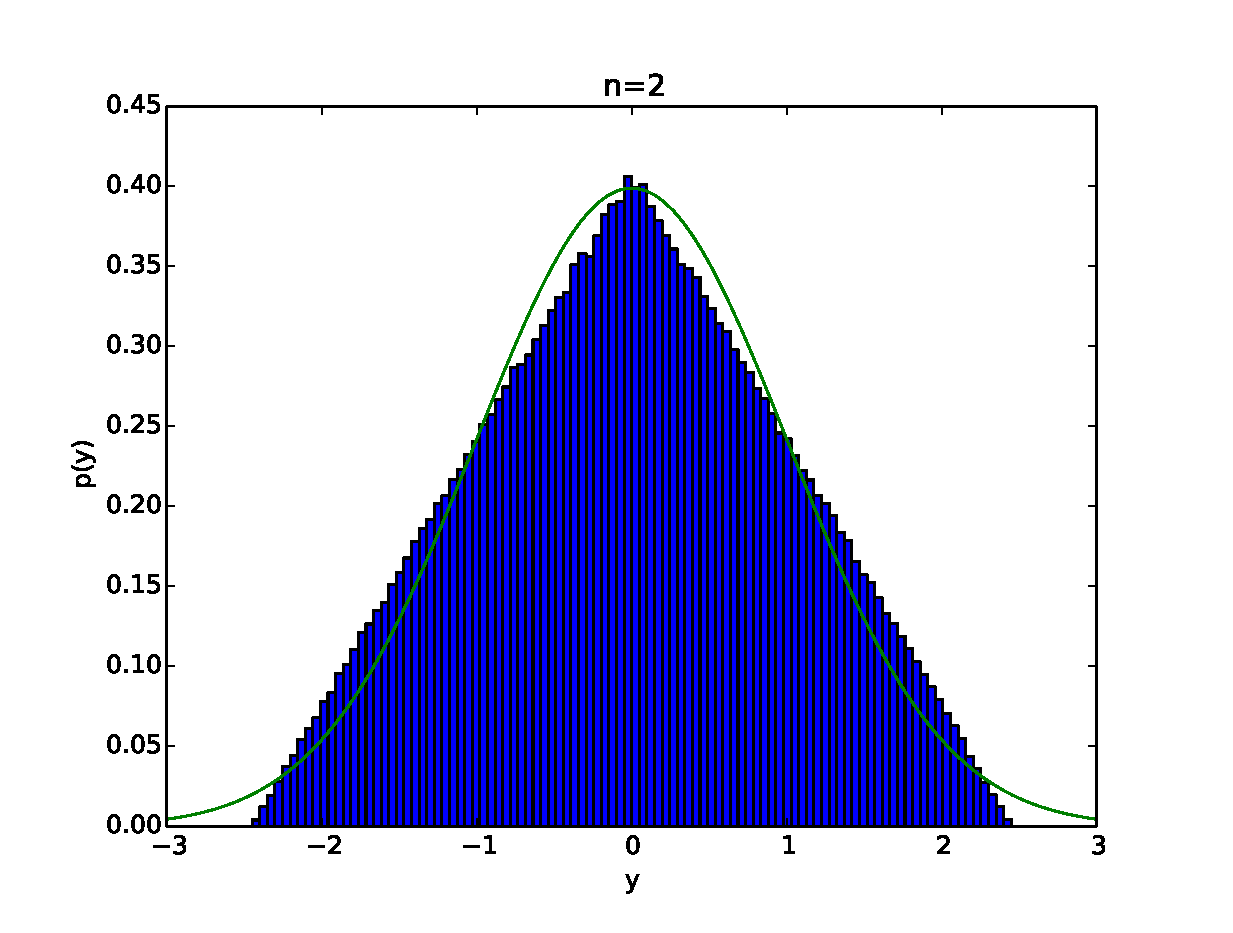
\includegraphics[width=0.5\linewidth]{clt1.eps}
}
\end{figure} 
\end{frame}

\begin{frame} 
  \begin{figure}[htp]
\mbox{
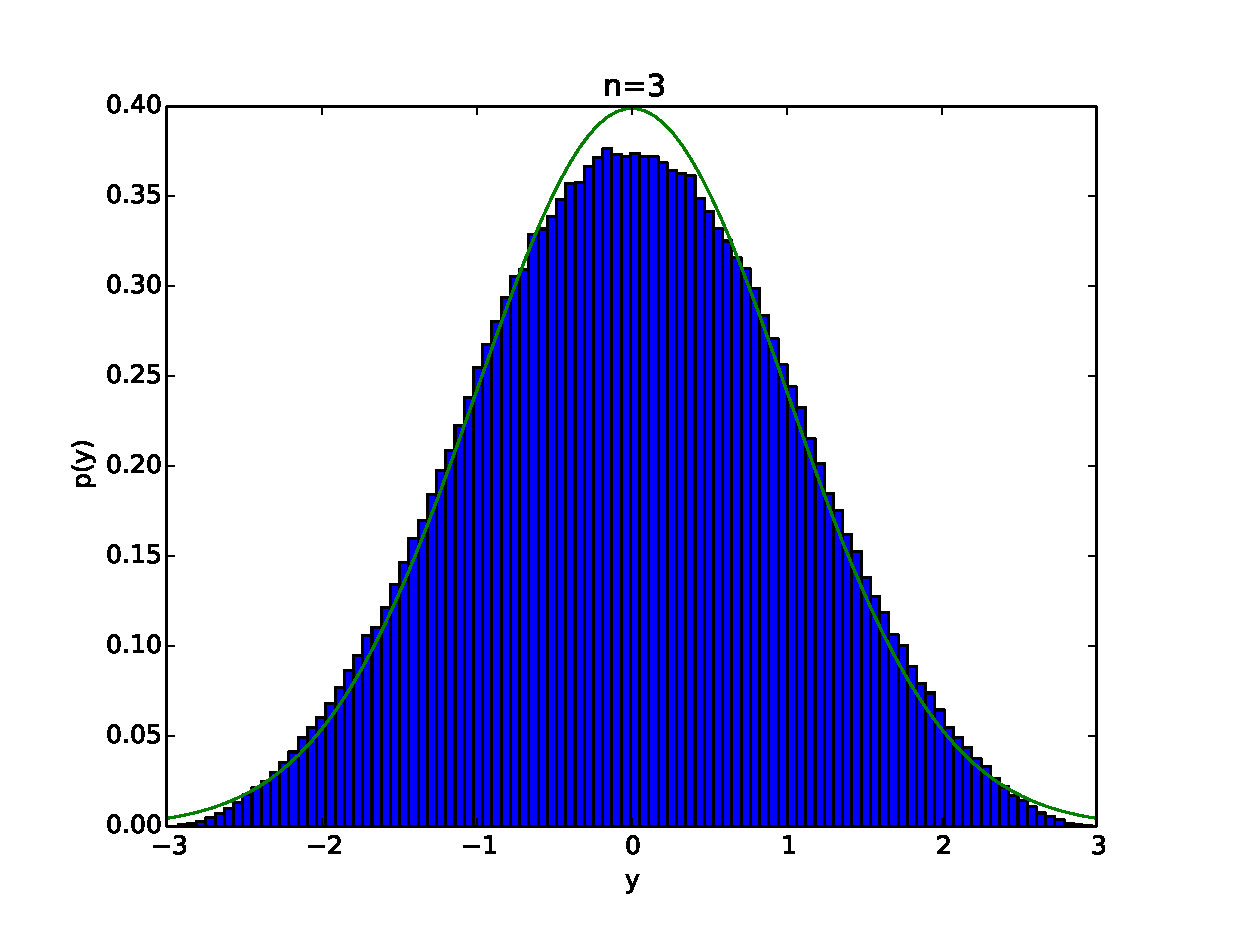
\includegraphics[width=0.5\linewidth]{clt2.eps}
}
\end{figure} 
\end{frame}


\begin{frame} 
  \begin{figure}[htp]
\mbox{
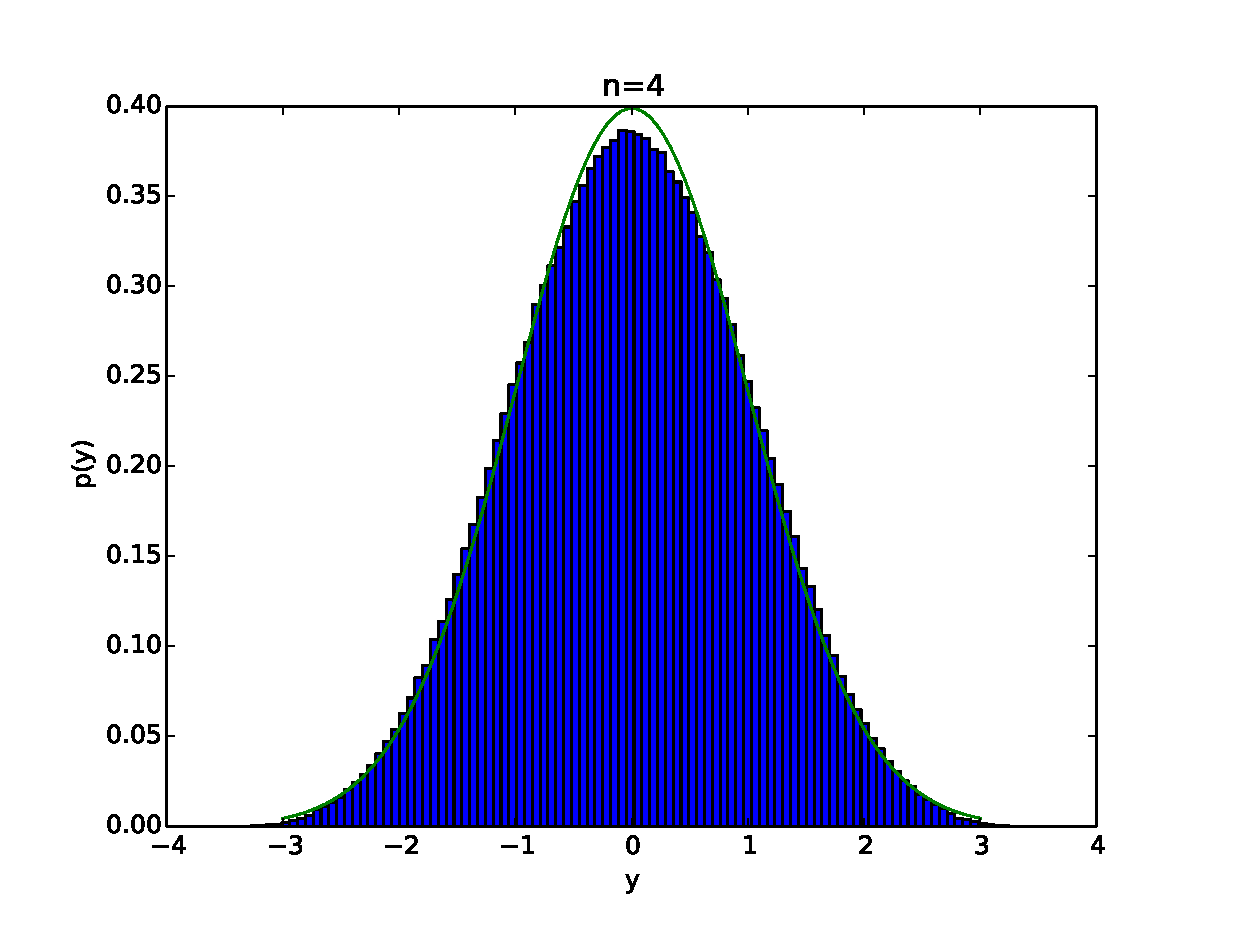
\includegraphics[width=0.5\linewidth]{clt3.eps}
}
\end{figure} 
\end{frame}

\begin{frame}{Exercise}  
\begin{itemize} 
 \item Let $X_1, X_2, \ldots X_n$ be a sequence of independent Bernoulli random variables with parameter $p = \frac{1}{2}$. Use the central limit theorem to derive an approximate \emph{distribution} for the mean of the first $100$ items of the sequence. 
  \item Let $Y$ be a binomial random variable with parameters $n=100$ and $p = \frac{1}{2}$. Using the Central Limit Theorem, show that a normal random variable X with mean $\mu =50$ and variance $\sigma^{2}=25$ can be used as an approximation of $Y$. 
\end{itemize}
\end{frame}




\begin{frame}{Summary} 
\begin{itemize} 
 \item There are different ways to characterise convergence of random variables 
 \item Strong law of large numbers says the sample mean of a set of observations converges to expectation 
 \item Central limit theorem 
\end{itemize}
 
\end{frame}


\end{document} 